\section{Durchführung}
\subsection{Versuchsaufbau}
Der Aufbau des Versuchs kann anhand des Fotos in Abbildung $\ref{fotosaufbau1}$ nachvollzogen werden.

\begin{figure}[H]
  \centering
  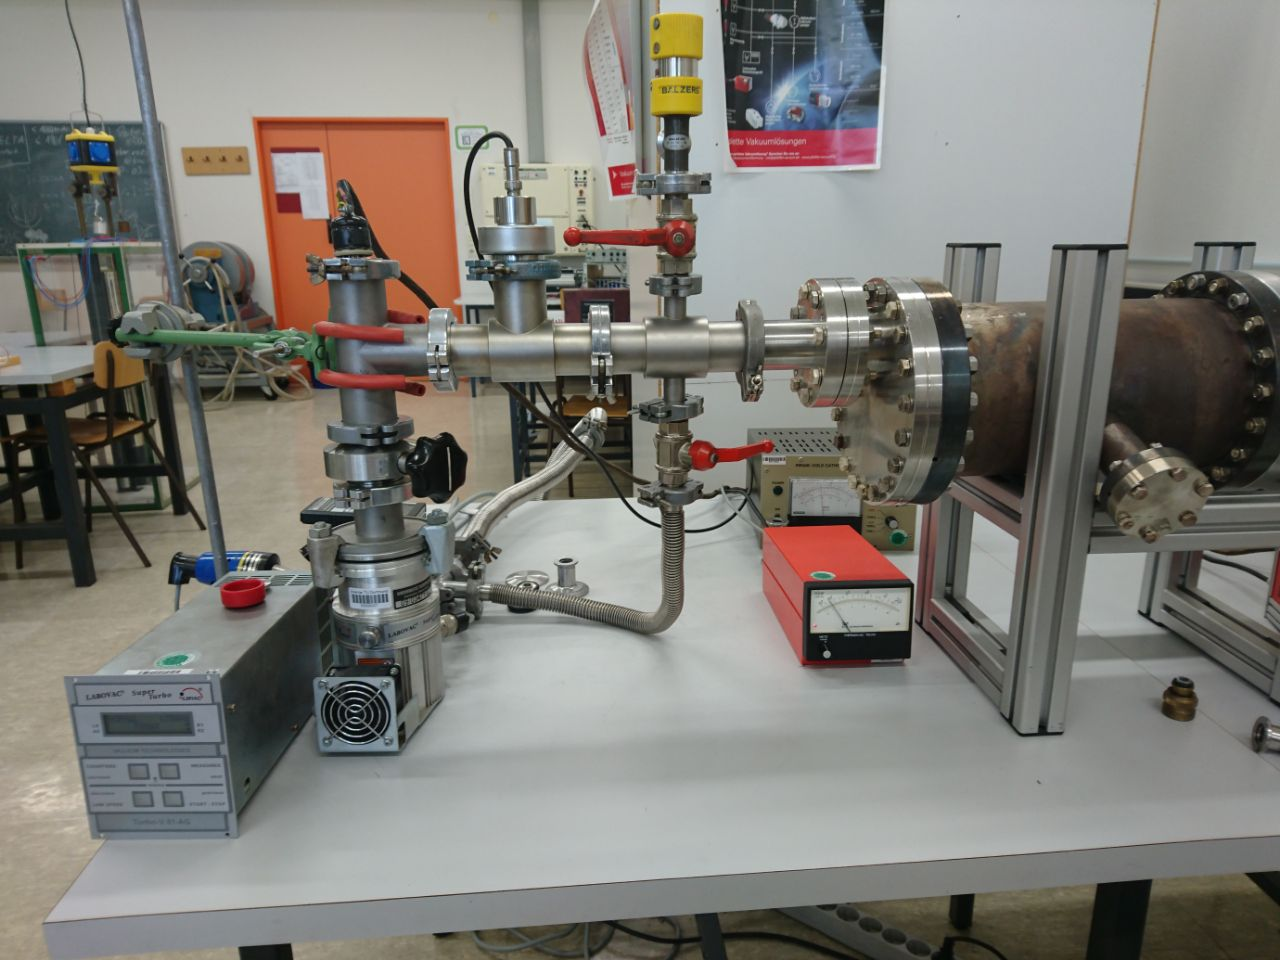
\includegraphics[scale=0.2]{Bilder/Versuch2.jpg}
  \caption{Frontansicht des Versuchaufbaus.}
  \label{fotosaufbau1}
\end{figure}
Zur besseren Übersicht befindet sich des Weiteren ein schematischer Aufbau des Versuchs in Abbildung $\ref{aufbauschema}$.
\begin{figure}[H]
  \centering
  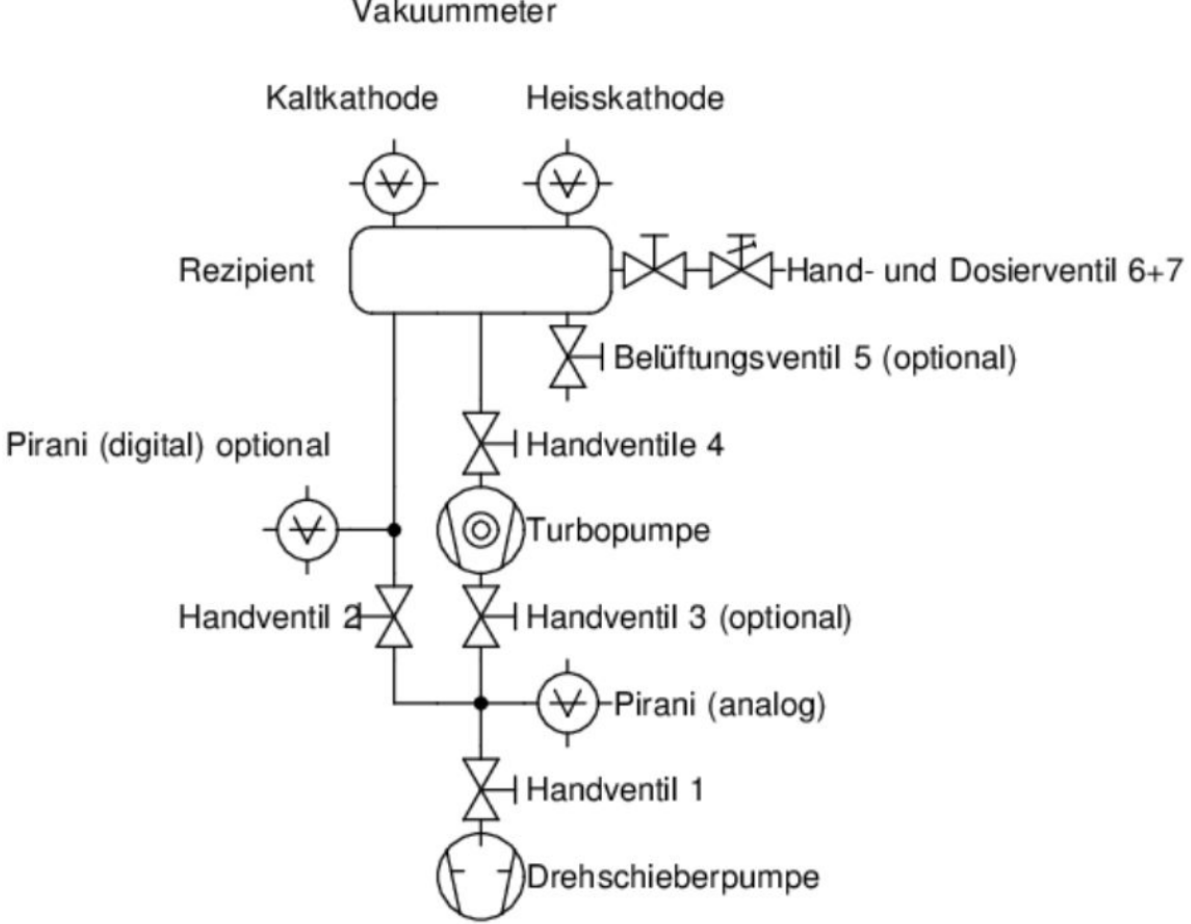
\includegraphics[scale=0.4]{Bilder/schemaVersuch.png}
  \caption{Schematische Darstellung des Versuchsaufbaus.\cite{anleitung}}
  \label{aufbauschema}
\end{figure}
\subsection{Versuchsdurchführung}
Zu Beginn des Versuchs wird die Dichtigkeit des Aufbaus getestet. Hierzu wird zunächst mit der Drehschieberpumpe ein Vorvakuum von höchstens $0,05$\,\si{\milli\bar} erzeugt. Wenn der nötige Druck erreicht
ist, wird die Turbomolekularpumpe hinzugeschaltet und der Gasdruck auf höchstens $8 \cdot 10^{-5}$\,\si{\milli\bar} gesenkt. Ist dies möglich, so gilt der Aufbau als dicht.\\
Vor Beginn der Messung ist es außerdem notwendig, den Aufbau mit einem Heißluftfön zu erhitzen um Wasser aus dem Tank zu entfernen und Desorptionseffekte während den Messungen zu vermindern.
\subsubsection{Untersuchung der Turbomolekularpumpe}
Als erste Messung wird die Evakuierungskurve der Turbomolekularpumpe bestimmt. Hierzu wird die Drehschieberpumpe abgeschiebert (Ventil 2 geschlossen) und über das Nadelventil ein Gleichgewichtsdruck von
$8 \cdot 10^{-3}$\,\si{\milli\bar} eingestellt. Das Glühkathoden-Vakuummeter wird eingeschaltet. Nadel- und Kugelventil werden geschlossen und der Druck mit der Zeit aufgenommen. Es werden 5 solcher Messungen
durchgeführt.\\
Es wird außerdem eine Leckratenmessung vorgenommen. Hierzu wird mit dem Nadelventil ein Gleichgewichtsdruck eingestellt und daraufhin das Ventil zur Pumpe geschlossen. Es wird
der Druckanstieg mit der Zeit vermessen. Insgesamt sollen drei solcher Messreihen für vier verschiedene Werte durchgeführt werden.
\subsubsection{Untersuchung der Drehschieberpumpe}
Für die Drehschieberpumpe werden ebenfalls Evakuierungskurve und Leckrate untersucht. Für die Evakuierungskurve wird die Turbomolekularpumpe abgeschiebert (Ventil 3 und 4 schließen) und Ventil 2 geöffnet.
Das Handventil zur Drehschieberpumpe wird geschlossen und der Rezipient über Ventil 6 auf Normaldruck $(1000 \pm 100)\,  \si{mbar}$ belüftet. Die Messung beginnt, indem Ventil 6 geschlossen und das Handventil
möglichst zeitgleich geöffnet wird. Es wird der Druckabfall mit der Zeit aufgezeichnet.\\
Die Leckratenmessung verläuft hier analog zu der der Turbomolekularpumpe. Als Gleichgewichtsdruck werden  $p_G=0,1;0,4;0,8 \text{ und } 1 $\,\si{\milli\bar} eingestellt. Es werden jeweils drei Messungen
pro Gleichgewichtsdruck durchgeführt.\\
Wegen des höheren Druckes wird bei der Drehschieberpumpe das Pirani-Messgerät anstatt des Glühkathoden-Vakuummeters genutzt.
\newpage
